\section{Methodology}
\label{sec:methodology}


In this section, we first review the preliminaries of the Optimal Transport problem in Sec.~\ref{sec:optimal_transport}. Then we demonstrate how to first establish the token anchors in Sec.~\ref{sec:token_anchors} and formulate the token sets optimization strategy within intra- and inter-frame level to exploit the necessary local and global spatiotemporal contexts in Sec.~\ref{sec:spatiotemporal}, leading to compact yet effective video tokens reduction in a training-free manner. We provide an overview of our AOT in Fig.~\ref{fig:method}.


\begin{figure*}[t]
    \centering
    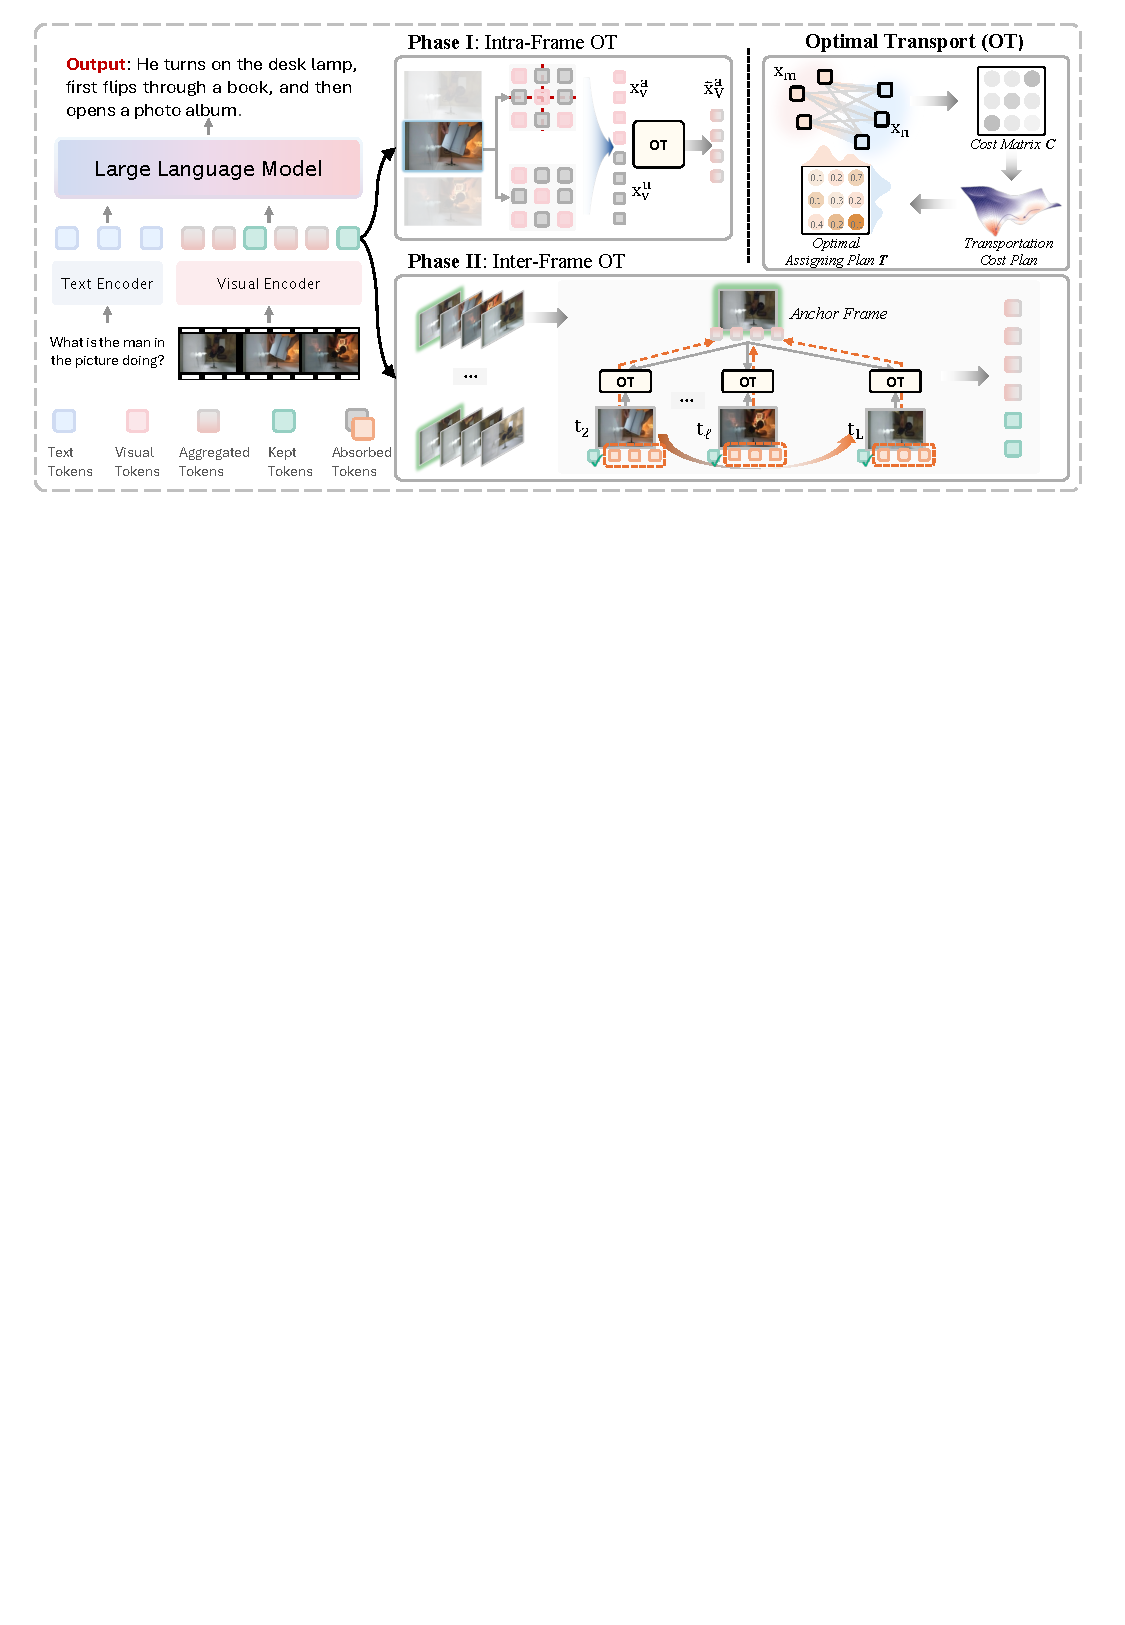
\includegraphics[width=\linewidth]{figs/cvpr26-token.pdf}
    \vspace{-0.6cm}
    \caption{Overall pipeline of our \textbf{AOT}. Our method compresses tokens of video LLMs across spatiotemporal through optimal transport, first establishing token anchors within each frame to cover semantically important and spatially diverse token candidates, then utilizing optimal transport to aggregate the necessary informative cues within Intra-Frame at phase I, and finally shifting the optimization strategy into temporal within Inter-Frame at phase II. The proposed AOT preserves both temporal and visual integrity by utilizing efficient Sinkhorn-Knopp Iteration to solve the optimal transport plan assignment.}
\label{fig:method}
% \vspace{-0.4cm}
\end{figure*}

\subsection{Optimal Transport}
\label{sec:optimal_transport}
% \vspace{-5pt}

Optimal transport~(OT) distance is a widely used metric for the comparison of distributions. Here, we only focus on the discrete situation which is more related to our pipeline. Assuming we have two sets of tokens (features), the discrete distributions are formulated as:

\begin{equation} 
\label{eq:discrete}
    U=\sum_{m=1}^{M}u_m\delta_{\bm{X}_m} \hspace{2em} \text{and} \hspace{2em} V=\sum_{n=1}^{N}v_n\delta_{\bm{X}_n},
\end{equation}
where $\bm{u}$ and $\bm{v}$ are the discrete probability vectors that sum to 1, and $\delta_{\bm{X}}$ is a Dirac delta function placed at support point $\bm{X}=\{X_1,...,X_N\} \in \mathbb{R}^{N \times d}$ in the visual token embedding space.
Then, the total distance is modeled as:
\begin{equation} 
\label{eq:cost}
    <\bm{T},\bm{C}> = \sum_{m=1}^{M}\sum_{n=1}^{N}\bm{T}_{m,n}\bm{C}_{m,n},
\end{equation}
We call $\bm{C}$ the cost matrix in which each point denotes the cost between $\bm{X}_m$ and $\bm{X}_n$, such as $\bm{C}_{m,n}= 1- \text{sim}(\bm{X}_m,\bm{X}_{n})$. While $\bm{T} $ is denoted as transport plan, which is learned to minimize the total distance. The optimization problem of optimal transport is formulated as:
\begin{equation} 
\label{eq:optimization}
    \begin{aligned}
        & d_{\text{OT}}(\bm{u},\bm{v}|\bm{C}) = \underset{\bm{T}}{\text{minimize}}
         <\bm{T},\bm{C}>, \\
        & \text{subject to}
        ~~~~~~\bm{T}\bm{1}_N = \bm{u},\; \bm{T}^\top \bm{1}_M = \bm{v},\; \bm{T} \in \mathbb{R}^{M \times N}_+.
    \end{aligned}
\end{equation}

As directly optimizing the above objective requires significant time-consumption, we apply the Sinkhorn distance~\citep{cuturi2013sinkhorn}, a fast iterative solution, to use an entropic constraint for fast optimization. The optimization problem with a Lagrange multiplier of the entropy
constraint is:
\begin{equation} 
\label{eq:Sinkhorn}
    \begin{aligned}
        & d_{\text{OT},\lambda}(\bm{u},\bm{v}|\bm{C})=\underset{\bm{T}}{\text{minimize}}
         <\bm{T},\bm{C}> - \lambda h(\bm{T}), \\
        & \text{subject to}
        ~~~~~~~\bm{T}\bm{1}_N = \bm{u},\; \bm{T}^\top \bm{1}_M = \bm{v},\;
        \bm{T} \in \mathbb{R}^{M \times N}_+.
    \end{aligned}
\end{equation}
where $h(\cdot) $ is entropy and $\lambda \geq 0$ is a hyper-parameter. Then we can have a fast and off-the-shelf optimization solution with a few iterations as:
\begin{equation} 
\label{eq:Sinkhorn_optimization}
    \bm{T}^*= \text{diag}(\bm{u}^{(t)}) \exp(-\bm{C}/\lambda) \text{diag}(\bm{v}^{(t)}),
\end{equation}
where $t$ denotes the iteration and in each iteration 
$\bm{u}^{(t)} =\bm{u}/\left((\exp(-\bm{C}/\lambda)\bm{v}^{(t-1)}\right)$ and  $\bm{v}^{(t)} =\bm{v}/\left((\exp(-\bm{C}/\lambda)^\top\bm{u}^{(t)}\right) $, with the initiation $\bm{v}^{(0)} = \bm{1}$.


\subsection{Local-Global Token Anchors Establishment}
\label{sec:token_anchors}

\noindent \textbf{Global Anchors.}
Given that the final layers of visual encoders capture global information, we follow recent works~\cite{zhang2024cls,yang2025visionzip} to select global tokens that receive the most attention from the [\texttt{CLS}] token $x_{[\mathtt{CLS}]}$ in the output layer.
%
%
Specifically, the [\texttt{CLS}] attention computation for each attention head can be represented by:
\begin{equation}
\label{eq:cls-attn}
    \begin{aligned}
        S_{[\mathtt{CLS}]}^h &= \mathtt{Softmax}\!\left(\frac{Q_{[\mathtt{CLS}]}K_V^\top}{\sqrt{D}} \right),
    \end{aligned}
\end{equation}
where $Q_{[\mathtt{CLS}]}$ and $K_V$ represent the query and key output for head $h\in [1, H]$, $D$ denotes the hidden state size, and $S_{[\mathtt{CLS}]}^h$ represents the [\texttt{CLS}] attention. Given the visual token sequence $X_V$, the global tokens are then selected by:
%
\begin{equation}
\begin{split}
    S_{[\mathtt{CLS}]}^{\texttt{avg}}
    &= \frac{1}{H} \sum_{h=1}^H S_{[\mathtt{CLS}]}^h,\\
    \mathbf{x}_{V}^{\mathtt{g}}
    &= \operatorname{TopK}\big(\mathbf{x}_V,\; S_{[\mathtt{CLS}]}^{\texttt{avg}},\; K\big),
\end{split}
\end{equation}
where $\operatorname{TopK}(\cdot)$ selects the $K$ visual tokens with the highest $S_{[\mathtt{CLS}]}^{\texttt{avg}}$ scores, yielding the final kept token set $\mathbf{x}_{V}^{\mathtt{g}}$ of size $K$. For LVLMs without a [\texttt{CLS}] token (\textit{e.g.,} SigLip~\cite{zhai2023sigmoid} and Qwen-2.5-VL~\cite{bai2025qwen2}), we similarly define token importance scores based on self-attention (\textit{i.e.,} the average attention each
visual token receives from others) and apply the same Top-$K$ selection.



\noindent \textbf{Local Anchors.}
To enable fine-grained local details preservation, we divide the image feature into $W$ non-overlapping grid-wise windows and select locally important tokens with the highest [\texttt{CLS}] attention from a shallow layer $l$ within each window, following~\cite{li2024llava,chen2024far,zhang2024llavanextvideo}.
Given a total local budget $K$, we allocate $K_w=K/W$
tokens per window and also perform Top-$K$ selection:
\begin{equation}
    \mathbf{x}_V^{\mathtt{l}}
    =
    \bigcup_{w=1}^W
    \operatorname{TopK}\big(
        \mathbf{x}_V^w,\,
        S_{[\mathtt{CLS}]}^{\texttt{avg}},\,
        K_w
    \big),
\end{equation}
where $\mathbf{x}_V^w$ denotes tokens in window $w$.
The final anchor set is the union of global and local tokens,
$\mathbf{X}_V^{\texttt{anchors}} = \mathbf{x}_V^{\mathtt{g}} \cup \mathbf{x}_V^{\mathtt{l}}$,
and the remaining tokens are denoted as
$\mathbf{X}_V^{\texttt{unanchors}}$.
Following~\cite{zhang2025vscan}, we balance global and local selection, \textit{e.g.,} $|\mathbf{x}_V^{\mathtt{g}}| = |\mathbf{x}_V^{\mathtt{l}}|$, and exclude locally selected tokens from the global set to avoid duplication and redundancy.



\subsection{Spatiotemporal Pruning}
\label{sec:spatiotemporal}

\noindent \textbf{Intra-Frame Pruning with OT.}
For each frame, given extracted visual tokens as $\bm{X}=\{X_1,...,X_N\} \in \mathbb{R}^{N \times d}$, we perform token anchors selection strategy above to establish $\mathbf{X}_V^{\texttt{acnhors}} \in \mathbb{R}^{M \times d}$ (dubbed $\mathbf{X}_V^{\texttt{a}}$) and $\mathbf{X}_V^{\texttt{unanchors}} \in \mathbb{R}^{(N-M) \times d}$ (dubbed $\mathbf{X}_V^{\texttt{u}}$). Built upon OT, we learn the geometric alignment transport plan $\bm{T}$ with these fixed support sets $\mathbf{X}_V^{\texttt{a}}$ and $\mathbf{X}_V^{\texttt{u}}$, by minimizing the following OT distance to push $\mathbf{X}_V^{\texttt{u}}$ to $\mathbf{X}_V^{\texttt{a}}$:
\begin{equation}
\label{eq:distance}
    \begin{aligned}
         d^{intra}_{\text{OT}}(k) = d_{\text{OT}}(\bm{u},\bm{v}|\bm{1}-\bm{{(X^a_V)}}^\top\bm{({X}^{u}_{V})}),
    \end{aligned}
\end{equation}
where $\bm{C}=\bm{1}-\bm{{(X}^a_V)}^\top\bm{({X}^{u}_{V})}$ denotes that we use the inverse cosine similarity distance between $\bm{X^a_V}$ and $\bm{X^u_V}$ as the cost matrix. Then we compute the solution of transport plan $\bm{T_{intra}}^*$ as Eq.~\ref{eq:Sinkhorn_optimization} and the final OT distance $d^{intra}_{\text{OT}}(k)$. Given the optimal transport plan $\bm{T_{intra}}^* \in \mathbb{R}_+^{(N-M)\times M}$ between
$\mathbf{X}_V^{\texttt{u}}$ and $\mathbf{X}_V^{\texttt{a}}$, we aggregate the unselected tokens onto the anchor tokens to obtain the compressed visual representation.
For the $j$-th anchor token, we first compute its received transport mass from all unselected tokens:
\vspace{-1mm}
\begin{equation}
    m_j \;=\; \sum_{i=1}^{N-M} T^*_{ij},
\vspace{-1mm}
\end{equation}
where mass denotes the supplied context units and then update the corresponding anchor by a mass-normalized OT aggregation from unselected tokens:
\begin{equation}
    \tilde{\mathbf{x}}^{a}_j
    \;=\;
    \frac{
        \mathbf{x}^{a}_j
        \;+\;
        \lambda_{intra} \sum_{i=1}^{N-M} T^*_{ij} \,\mathbf{x}^{u}_i
    }{
        1 \;+\; \lambda_{intra} m_j
    },
    \quad j = 1,\dots,M,
\end{equation}
where $\lambda_{intra}$ is a weighting coefficient for controlling the final contextual contribution to token anchors of the OT-based update. The final intra-frame compressed token set is then updated as:
\begin{equation}
    \tilde{\mathbf{X}}_V^{\texttt{a}}
    \;=\;
    \left\{\tilde{\mathbf{x}}^{a}_1, \dots,
    \tilde{\mathbf{x}}^{a}_M\right\}
    \in \mathbb{R}^{M \times d},
\end{equation}
which is used as the pruned visual tokens for the subsequent temporal pruning.




\noindent \textbf{Inter-Frame Pruning with OT.}
Beginning by segmenting the overall sampled frames into several frame clips which is adopted by uniform sampling or dynamic clustering, for each frame clip $\mathcal{C} = \{t_1,\dots,t_L\}$, we use the intra-frame compressed tokens of the first frame as temporal anchors:
\[
\mathbf{A}^{(1)} = \tilde{\mathbf{X}}^{\texttt{a}}_{V,t_1}
= \{\mathbf{x}^{(1)}_j\}_{j=1}^M.
\]
%
For each subsequent frame $t_\ell$ ($\ell = 2,\dots,L$), let
$\mathbf{S}^{(\ell)} = \tilde{\mathbf{X}}^{\texttt{a}}_{V,t_\ell}
= \{\mathbf{x}^{(\ell)}_i\}_{i=1}^{M}$ denotes its intra-frame
compressed tokens, and $\mathbf{A}^{(\ell-1)} = \{\mathbf{x}^{(\ell-1)}_j\}_{j=1}^{M}$ represents the current clip anchors after $(\ell-1)$ times OT aggregation across consecutive frames.
%
For each subsequent frame $t_\ell$ ($\ell=2,\dots,L$), with anchors
$\mathbf{A}^{(\ell-1)} = \{\mathbf{x}^{(\ell-1)}_j\}_{j=1}^{M}$ and
tokens $\mathbf{S}^{(\ell)} = \{\mathbf{x}^{(\ell)}_i\}_{i=1}^{M}$,
we further formulate the inter-frame OT distance using optimal transport as:
\begin{equation}
    d^{\text{inter}}_{\text{OT}}(\ell)
    =
    d_{\text{OT}}\!\left(
        \bm{u}, \bm{v}
        \,\big|\,
        \bm{1}
        -
        \big(\mathbf{A}^{(\ell-1)}\big)
        \big(\mathbf{S}^{(\ell)}\big)^\top
    \right),
\end{equation}
and obtain the inter-frame optimal transport plan as:
\begin{equation}
    \bm{T_{inter}}^{(\ell)\,*}
    =
    \mathrm{OT}\!\left(
        \bm{u}, \bm{v}
        \,\big|\,
        \bm{1}
        -
        \big(\mathbf{A}^{(\ell-1)}\big)
        \big(\mathbf{S}^{(\ell)}\big)^\top
    \right),
\end{equation}
where this also utilizes a fast Sinkhorn-based solver similar to the intra-frame scenario. We then apply normalization along the row of $\bm{T_{inter}}^{(\ell)\,*}$ to get the assignment probabilities,
\begin{equation}
    p^{(\ell)}_{ij}
    =
    \frac{T^{(\ell)\,*}_{ij}}{\sum_{j'} T^{(\ell)\,*}_{ij'}},
    \qquad
    q^{(\ell)}_i = \max_j p^{(\ell)}_{ij},
\end{equation}
which are used to decide whether a token is aggregated into anchors
who showcases potential similar visual content or kept as a temporally variant token to maintain dynamics.
Specifically, if $q^{(\ell)}_i < \tau$, the $i$-th token of frame $t_\ell$
is considered having drastic temporal change and kept as usual; otherwise, it is smoothly aggregated into the current clip anchors analogous to intra-frame pruning optimization:
\begin{equation}
    \mathbf{a}^{(\ell)}_j
    =
    \frac{
        \mathbf{a}^{(\ell-1)}_j
        +
        \lambda_{inter}
        \sum_{i:\,q^{(\ell)}_i \ge \tau}
        p^{(\ell)}_{ij}\,\mathbf{s}^{(\ell)}_i
    }{
        1
        +
        \lambda_{inter}
        \sum_{i:\,q^{(\ell)}_i \ge \tau}
        p^{(\ell)}_{ij}
    },
    \quad j=1,\dots,M.
\end{equation}
By iterating this procedure over frames in the clip, we obtain
one compact set of clip-level anchors (from $\mathbf{A}^{(\ell)}$) along with a small number of remaining high-change tokens, which together facilitate the spatiotemporal pruned visual tokens.
The proposed AOT obtains necessary local-global semantic and context aggregation across spatiotemporal dimensions by adopting optimal transport to assemble informative cues from low-discriminative or relatively similar tokens under removing or merging. Our method considers their intrinsic contributions to the compact token anchors which globally abstracts and compresses spatiotemporal redundancy and retains essential temporal dynamics, significantly accelerating Video LLM inference while preserving both temporal and visual integrity. Meanwhile, optimal transport solution can be quickly and efficiently solved by the off-the-shelf Sinkhorn-Knopp Iteration~\cite{cuturi2013sinkhorn} with negligible computation overhead, leading to an efficient and effective training-free manner.

